\subsection{Forside}
\label{subsec:brug-forside}

Når man taster sig ind på hjemmesiden \url{http://foodl.dk}, bliver man mødt af en velkomsthilsen, der meget kort beskriver hjemmesidens formål og brug, som kan ses på \figref{fig:overblik-forside}. Denne hilsen kan brugeren vælge at lukke ned. En cookie bliver gemt i browseren, så velkomsthilsnen ikke bliver vist igen, medmindre browserhistorikken bliver ryddet.

\begin{figure}[H]
	\centering
	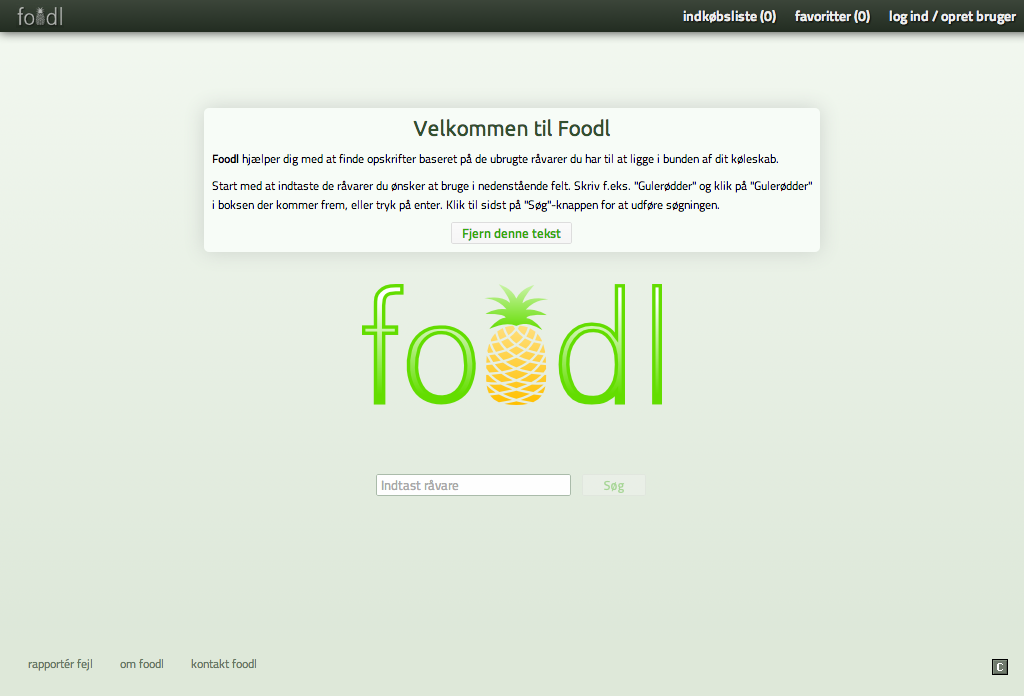
\includegraphics[scale=0.3]{billeder/foodl/thumbnails/forside.png}
	\capt{Denne figur har til formål at give et overblik over systemets forside.}
	\label{fig:overblik-forside}
\end{figure}

Navnet \Foodl{} er også en del af webapplikationens logo. For at gøre det klarere for en ny bruger, hvad siden handler om, erstattede vi et ``O'' i navnet med en stor ananas, fordi det er noget, der kan spises, og sidens formål er at give folk mulighed for at genbruge deres madrester. 

På toppen af alle undersider af \Foodl{} er det muligt at tilgå sidehovedet. Her er der mulighed for at navigere tilbage til forsiden ved at klikke på den mindre version af det logoet. Derudover kan man tilgå både en indkøbsliste, der er nærmere beskrevet i \secref{subsec:brug-indkoebsliste}, og en liste af favorit-opskrifter, som brugeren selv vælger fra hjemmesiden. Favoritlisten bliver beskrevet nærmere i \secref{subsec:brug-favoritliste}. Både indkøbslisten og favoritter har et tal i parentes, der fortæller brugeren, hvor mange varer, der er i den nuværende indkøbsliste, eller hvor mange opskrifter, der er gemt under favoritter. Dette kan ses på toppen af \figref{fig:overblik-forside}. På sidehovedet kan man også logge ind i systemet eller oprette en bruger, hvilket er forklaret nærmere i \secref{subsec:brug-opret}.

Efter brugeren føler sig tryg ved hjemmesiden og evt.\ har lukket velkomsthilsnen ned, så er det tid til at indtaste alle de råvaretyper, der ønskes brugt til madlavningen. Figur \ref{fig:foodl-soegefelt} viser, hvordan en sådan søgning foregår. Der bliver løbende indtastet bogstaver, og systemet undersøger for dele af tekststrenge, der matcher det, som bliver indtastet. Ud fra disse match gives der forslag til hvilke råvaretyper, man kan vælge. Man kan ikke indtaste, hvad som helst som et søgekriterie i systemet. Der er en lang række råvaretyper at vælge imellem. Hvis der \fx bliver indtastet kød i søgefeltet, så kommer der en liste af matchende råvaretyper som forslag, se \figref{fig:foodl-soegefelt}. Der er ingen begrænsning for, hvor mange råvaretyper, der kan indtastes som søgekriterier.

\begin{figure}[H]
	\centering
	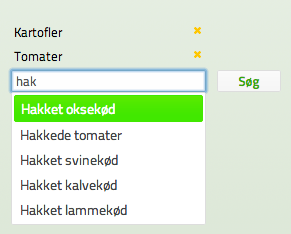
\includegraphics[scale=0.6]{billeder/foodl/soegefelt.png}
	\capt{Denne figur viser systemets søgefelt.}
	\label{fig:foodl-soegefelt}
\end{figure}


For at fuldføre en søgning skal man blot trykke på ``Søg'', der er til højre for søgefeltet. Når brugeren trykker ``Søg'', så arbejder systemet på at finde alle de opskrifter, der minimum har én ingrediens, der matcher en af de indtastede råvaretyper. Det er efter sådan en søgning, at brugeren finder ud af, hvad der er muligt at lave ud fra de råvaretyper, der er til rådighed (resultatet er afgrænset til den database, man har over opskrifter).
